% APORIA 2025
% For licence: see LICENSE

\documentclass[twoside]{book}

\title{Aporia 25 Feminist Edition}
\author{University of St Andrews Philosophy Society}
\date{2025}

% Paper size and margins
\usepackage[
    a4paper,
    outer=1.625in,
    inner=1.125in,
    top=1.5in,
    bottom=1.5in
]{geometry}
% Fonts
\usepackage{ebgaramond-maths}
\usepackage{amssymb}                    % Math symbols (e.g. therefore)
\usepackage{enumitem}                   % indenting next line of list
\usepackage[scale=0.78]{plex-mono}      % Monospace font
\usepackage[T1]{fontenc}                % T1 character encoding
\usepackage{microtype}
\usepackage{hanging}                    % For bibliographies
\usepackage{ragged2e}
% Columns
\usepackage{multicol}
% Include PDFs
\usepackage[final]{pdfpages}
% Links
\usepackage[anythingbreaks]{breakurl}
\usepackage[hyphens]{url}
\usepackage{hyperref}
\hypersetup{
    colorlinks,
    linkcolor={red!50!black},
    citecolor={blue!50!black},
    urlcolor={blue!80!black}
    }
\urlstyle{tt}
% Headers
\usepackage{fancyhdr}
% Headings
\usepackage[raggedright]{titlesec}
% for cftchapleader and cftdotsep in Table of Contents
\usepackage{tocloft}
% for WithSuffix
\usepackage{suffix}
% for list processing tools
\usepackage{etoolbox}

% Gap definitions
\def \hangingindent {3em}
\def \credgap {15pt}
\def \ackgap {10pt}
% Table of contents
%   depth = 0 ; only display article entries in ToC (not other
%   headings)
\setcounter{tocdepth}{0}
%   dots in the listing for chapters
\renewcommand{\cftchapleader}{\cftdotfill{\cftdotsep}}
% Heading styles
\renewcommand\thesection{\arabic{section}}

\titleformat{\chapter}[display]{\sffamily\LARGE\bfseries\raggedright}{}{0em}{}
\titlespacing*{\chapter}{0pt}{-50pt}{40pt}
\titleformat{\section}{\large\bfseries\raggedright}{{\sf\thesection}}{2em}{}
\titleformat{\subsection}{\bfseries}{{\sf\thesubsection}}{1.5em}{}
% Save this as default, so it can be revoked and restored
\let\sectionDefault\section
\let\titleformatDefault\titleformat

% Header style
\pagestyle{fancy}
\renewcommand{\chaptermark}[1]{%
\markboth{#1}{}}
\renewcommand{\headrulewidth}{0pt} % remove line under header
\fancyhead{}
\fancyhead[RO]{\small\sc\itshape\leftmark}
\fancyhead[LE]{\small\sc Aporia --- Feminist Ed. Vol. 25}
\fancyhead[RE]{\small\sc\itshape\leftmark}
\fancyhead[LO]{\small\sc Aporia --- Feminist Ed. Vol. 25}

% Define chapterauthor
\newcommand\chapterauthor[1]{\authortoc{#1}\printchapterauthor{#1}}
\WithSuffix\newcommand\chapterauthor*[1]{\printchapterauthor{#1}}
\makeatletter
\newcommand{\printchapterauthor}[1]{%
    {\parindent0pt\vspace*{-25pt}%
    \linespread{1.1}\large\scshape#1%
    \par\nobreak\vspace*{35pt}}
    \@afterheading%
}
\newcommand{\authortoc}[1]{%
    \addtocontents{toc}{\vskip-00pt}%
    \addtocontents{toc}{%
        \protect\contentsline{chapter}%
        {\hskip1.3em\mdseries\scshape\protect\normalsize#1}{}{}}
    \addtocontents{toc}{\vskip5pt}%
}
\makeatother
% Define acknowledgementlist
\makeatletter
\newcommand\acknowledgementlist[1]{%
    \forcsvlist{\acknowledgementlist@item}{#1}
}
\newcommand\acknowledgementlist@item[1]{
    \noindent#1%
    \par
    \vspace{\credgap}
}
\makeatother
% Define refsection
\def \refsection {\newpage\section*{Bibliography}}

% MAIN
\begin{document}
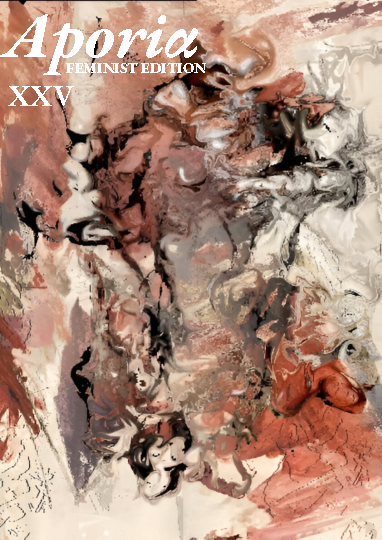
\includepdf{COVER.pdf}
\thispagestyle{empty}
\frontmatter
\begin{center}
    \vspace*{7cm}
    
    {\huge\textit{Aporia}}

    \vspace{1cm}

    {large The Feminist Edition}

    \vspace{3cm}
    \normalsize
    Undergraduate Journal of the St Andrews Philosophy Society

    \vspace{1cm}
    VOLUME XXV
\end{center}

\vfill 

\noindent \textit{Aporia} is funded by the University of St Andrews Philosophy
Society, which receives funds from the University of St Andrews
Department of Philosophy, the University of St Andrews Students’
Association, and independent benefactors.

\vspace*{\credgap}
{\noindent\LARGE\sc Letter from the Editor}
\vspace{\credgap}

\vspace{\ackgap}\noindent
Dear reader,

\vspace{\credgap}\noindent
As my work on this year’s Feminist Edition comes to an end, it is
tempting to speak of it only fondly. After all, as a philosopher, it
has been an intensely joyful experience to work with such a talented
team of editors, writers and philosophers to produce this year’s
edition.

However, as a feminist academic, this year has been challenging.
Misogyny and gendered violence against women are on the rise, and
academic work studying women’s health, lives and experiences is being
defunded, censored and framed as ‘frivolous’ or ‘unnecessary’. It is
not. This work – our work as feminist philosophers - undergirds
general feminist efforts in an essential way. It grants us the
theoretical tools to grapple with viscerally real problems, and it
therefore is in times like these that our research matters most.

As such, I would like to extend my immense gratitude to all the
philosophers who submitted their research and writing to The Feminist
Edition this year, as well as my congratulations to those who were
published. Your inquiry matters, and I am very proud to have worked to
provide a platform where your thoughts can be shared.

I also deeply thank this year’s editorial team, with a special tip of
the hat to my highly skilled colleagues Kirsty Graham and Joe
Bradstreet. You have all volunteered your time and brains over the
course of this year towards the noble cause of platforming young
academics and helping them develop their philosophical acumen. Thank
you so much for your hard work – it makes a difference.

Lastly, like last year, I want to express my gratitude to – and awe
for - all the inspiring women and feminist academics in the Philosophy
Society as well as the St Andrews Philosophy Department. To be
surrounded by you all is all the affirmation needed to know that what
we are doing here is worthwhile, and an academic necessity.

If you made it this far, I must also say – it is with great sadness I
now leave The Feminist Edition behind, but with great joy I leave it
in very competent hands. I cannot wait to see what the future holds
for this journal and the people who work so hard to bring it forth.

\vspace{\credgap}\noindent
Signing off,

\vspace{\ackgap}\noindent
Christina Landys Herre

\noindent
Editor-in-Chief, \emph{Aporia: The Feminist Edition}

\vspace*{\credgap}
{\noindent\LARGE\sc Acknowledgements}

\vspace*{\fill}
\begin{multicols}{2}
{\noindent\Large\sc Editors}
\vspace{\credgap}

\acknowledgementlist{
    Aliza Ashraf,
    Beth Cook,
    Maria de Feo,
    Ella Johnston,
    Hanaa Khan,
    Krisztian Kos,
    Zack Ledesma,
    Nawal Mirza,
    Claire Mizrahi,
    Phoebe Ray,
    Nathalie Rogers,
    Rosa Velasco Saavedra,
    Jacob Walchuk,
    Hoochang Yi
}
\columnbreak
\vspace*{\fill}
\acknowledgementlist{
Christina Landys Herre\newline\emph{Editor-in-Chief},
Mohit Agarwal\newline\emph{Technical Officer}
}
\vspace*{\fill}
\acknowledgementlist{
Ella Johnston\newline\emph{Cover Artist}
}
\end{multicols}
\vspace*{\fill}

\tableofcontents
\thispagestyle{empty}

\mainmatter

\chapter{Why Women and Men Cannot Love Each Other (Yet)}
\chaptermark{Why Women and Men Cannot Love Each Other}
\chapterauthor{Audrey Rodriguez,
\textit{University of Miami}}

% makes the section numbers roman numerals
\renewcommand{\thesection}{\Roman{section}}

% makes the subsection letters
\renewcommand{\thesubsection}{\alph{subsection}.}

\begin{quote}
In a heteronormative society, men and women are
typically expected to look not for authentic love, but simply a partner
of the opposite gender. This compulsory heterosexuality, as explained by
Adrienne Rich, and the resultantly tainted love story problematize views
about love like Berit Brogaard's ``appraisal respect''. I take Brogaard
to give an apt account of what we should want authentic love to be, one
in which we are said to love another when we properly evaluate their
role as a lovable lover. However, because loving another and evaluating
their lovability are not the goals of love as it stands, heterosexual
men and women cannot be said to love in the way Brogaard rightly
champions. Authentic love is then something most do not generally
experience, but all (who are interested in engaging in romantic love)
ought to strive for. I ultimately claim that developing respect for
ourselves, our peers, our same-sex relationships, and love itself are
the best ways for us to make authentic love widely accessible.
\end{quote}

\vspace{\credgap}

\noindent In a heteronormative society, men and women are
typically expected to look not for authentic love, but simply a partner
of the opposite sex. Can you be said to love your partner without truly
getting to \emph{choose}\footnote{My argument throughout this work pressupposes at least a minimal amount of free will. What authentic love would look like in a hard determinist picture is an interesting question, but whose answer is opaque enough that I will not be endeavoring to answer it here.} your partner? Many feminist theorists
have taken issue with whether men can love women under patriarchy since
patriarchy does not see women as ends-in-themselves, but the reverse
case has rarely been considered.

I argue that women are also not taught to strive to love men, but taught
to objectify men as a means to the securing of connection to a
subjectivity. Heterosexual love is thus an inauthentic experience for
heterosexual men and women alike. This is because heterosexual love
projects, as they stand, necessarily hold not love as their purpose; but
rather the fulfillment of societal expectations.

In Section I of this paper, I will explain the constraints compulsory
heterosexuality places on love. In Section II, I will recount Berit
Brogaard's framework describing romantic love as a goal-oriented emotion
that is importantly different from friendship\footnote{Throughout this
  paper I will refer to ``platonic love'' as ``friendship love'' in
  keeping with the terminological choice of one of the main authors with
  whose work I am interacting, namely, Berit Brogaard (2022). Any
  instance of ``friendship love'' can be understood to refer to the same
  love between friends that the phrase ``platonic love'' picks out.}
love. I will use the problem of compulsory heterosexuality to complicate
Brogaard's assumption that the appraisal of one's performance in the
role of lover accounts for lovers' ability to respect each other when
engaging in romance is generally possible.

It will become clear that most do not yet have the type of respect
necessary to be said to love authentically, and in Section III I will
argue that men and women cannot generally love each other in an
authentic sense. I will use the phrases ``genuine love''\footnote{Bauer,
  Nancy. \emph{Simone de Beauvoir, Philosophy, \& Feminism}. New York:
  Columbia University Press, 2001. 164-165.} and ``authentic
love''\footnote{Bauer,  Nancy. \emph{Simone de Beauvoir, Philosophy, \& Feminism}. New York: Columbia University Press, 2001. 164.} interchangeably to refer to a love that
is genuine/authentic in so far as it ``is an expression of the highest
of moral laws: when I love another person genuinely I both exercise my
existential freedom and evince the highest respect for the freedom of
other, on which, I understand, my own freedom rests.'' (Bauer, 164--5)
This respect for another's freedom is something I take to be most
clearly portrayed by Brogaard's lovability account, and something that
clearly seems to be a necessary aspect of a kind of love worth having.
These oppressive societal constraints also make heterosexual friendship
love generally impossible according to the ``appraisal respect''
standard. Finally in Section IV, I will consider general objections to
my claims, offer responses, and consider ways in which we could
eventually create the conditions for and ultimately secure an authentic
heterosexual love.

\section{Compulsory Heterosexuality}

Adrienne Rich writes in her essay ``Compulsory Heterosexuality'' that
heterosexuality is a ``\emph{political institution}'' that dictates that
women must be attracted to and pursue relationships with men so as to
assure the ``male right of physical, economical, and emotional access''
to women.\footnote{Rich, ``Compulsory Heterosexuality and Lesbian
  Existence.'' 647.} To deny patriarchy's requirement of heterosexual
love from women is often to open oneself up to ``physical torture,
imprisonment, psychosurgery, social ostracism, and extreme
poverty.''\footnote{Rich, ``Compulsory Heterosexuality and Lesbian
  Existence.'' 653.} Heterosexuality is then required of
women not only at threat of discomfort while in the confines of
patriarchy, but at the risk of a woman's mental, social, and physical
safety. All those who live under patriarchy are indoctrinated to believe
the only form of romantic love that is common, ``normal,'' or worthy is
heterosexual in nature.

The coercive power of this expectation of heterosexuality is so strong,
in fact, that it becomes completely compulsory. With the compulsion of
heterosexuality in romantic love, and the definition of romantic love
thus being inextricable from a heterosexual relationship structure, this
means love itself becomes compulsory as does its structure. One cannot
be said to truly be making a choice when only given one option, and one
cannot be said to truly engage in loving when only given one definition
and version of love. Therefore, those in most heterosexual relationships
cannot be said to truly be loving. Instead, many are unwittingly
engaging in a societally mandated project akin to military enlistment.

\subsection{Why Heterosexual Love is In Question}

Heterosexual love is forced in a way most other types of love are not. I
have been asked many times why I take most issue with heterosexual love
if starting from an asymmetry in respect or societal power. There are
many romantic relationships that can span any number of other oppressed,
or not oppressed, lines - be these racial, socioeconomic, in terms of
age, etc. I believe many of these are a non-issue in the face of the
account of an ideally respectful love I sketch in Section III.
Addressing the other types of love that still might be questionable even
in the face of such an authentic love is out of the scope of this paper.
Women\footnote{Throughout this paper I will use the terms ``women'' and
  ``men'', and will take both to mean anyone who identifies as either of
  those two genders at least occasionally. Again, there are many
  identity markers that might call for a more fine-grained and specific
  discussion that considers more than just the issues in love between
  binary genders. It is just the general power imbalance between those
  who identify as men and those who identify as women, and the
  compulsory nature of heterosexuality, that I think makes heterosexual
  love one of the most contentious and confounding forms of romantic
  love.} are understood by most to be pervasively defined in terms of
men and generally oppressed by the objectifying structure of this
relation. In the next two Sections I will try to make clear how such a
societal power imbalance and compulsory heterosexuality clearly
problematize heterosexual love given the world as it is now.

The realization of male sexual power ``by adolescent boys through the
social experience of their sex drive'' is the same realization that
causes ``girls [to] learn that the locus of sexual power is
male.''\footnote{Rich, ``Compulsory Heterosexuality and Lesbian
  Existence.'' 645.} Girls come to know their sexual identities through
boys' realization of theirs, making female sexual desire compulsorily
linked to that of men and pleasing men. In a search for any kind of
negotiating power on the societal stage, women become sexual responders
to male power as opposed to explorers and actors of their own desires.
This is all true if one accepts, as many feminists do, that women are
kept subordinate by oppressive structures by patriarchy at best, or that
women are entirely second-class citizens in how they are respected by
societies at large and at worst. Not only are women taught to define
themselves in terms of their ability to appeal to men's sexual appetite,
but they also come to know themselves as objects.

It is in the packaging of heterosexual love in the ``workplace [\ldots]
where women have learned to accept male violation of our psychological
and physical boundaries as the price of survival; where women have been
educated---no less than by romantic literature or by pornography---to
``perceive ourselves as sexual prey.''\footnote{Rich, ``Compulsory
  Heterosexuality and Lesbian Existence.'' 642.} All cultural and
political channels create and fortify compulsory heterosexuality, making
it a cultural and political pillar itself. This enforced and thusly
reinforced self-perception of women as sexual prey causes women to feel
that danger at the hands of men is imminent and the only remedy is
aligning themselves with men in the hopes of being protected.

Rich asks that all women who assume heterosexuality to be innate or a
choice consider that it is in fact ``something that has to be imposed,
managed, organized, propagandized, and managed by force.''\footnote{Rich, ``Compulsory
  Heterosexuality and Lesbian Existence.'' 648.} Heterosexuality is thus not a choice or preference, but
rather it is a regime backed by threat of death, torture, and social
abandonment.

Love and this sexual power imbalance cause women enveloped by compulsory
heterosexuality to see their identity fulfill ``a secondary role and
[grow] into male identification.''\footnote{Rich, ``Compulsory
  Heterosexuality and Lesbian Existence.'' 642.} Female
subordination is then eroticized and the ``access to women only \emph{on
women's terms}'' becomes something unthinkably frightening to
men.\footnote{Rich, ``Compulsory
  Heterosexuality and Lesbian Existence.'' 643.} It is this identification with men, fear of
societal retaliation, and the eroticization of female subordination that
makes women search for themselves by way of being romantically
associated with a man. A woman's difficulty in separating her sexual
drive from that of men becomes part of the love and sex game, with women
having to become accustomed to relinquishing their power of desire to
men. This results in a clear objective laid out for women in engaging in
romantic projects\footnote{I elect to use the term ``romantic projects''
  instead of ``romantic relationships'' because I do not want to confuse
  relationship projects with romantic ones. It seems the former would
  need to factor in more practical matters (longevity of the
  relationship, living arrangements, etc.) than I have space to
  undertake in this project. I would like to leave the definition of
  what a romantic relationship is and questions regarding polyamory and
  how much ``committed'' ``monogamy'' is indicative of a healthy
  relationship open. I merely mean to argue throughout this paper that
  heterosexual love is misunderstood and inappropriately portrayed on a
  societal scale and has little to no authenticity motivating it.}:
securing a subjectivity to which you can attach yourself. This
objectifies men because they become the kind of object, the kind of
thing, that has the kind of subjectivity needed to live more freely, and
women are taught they can only really find power and identity by growing
into a male's identity since their sexual desires and others are defined
in terms of men's desires. Thus, romantic projects are the clearest way
for women to gain societal power and ``love'' so-construed never figures
into the picture.

\section{Love for Lovability's Sake}

Compulsory heterosexuality will thus be the lens through which we come
to understand love, and Berit Brogaard's definition of love will give a
theory to be considered. It is necessary to give a definition of love
that can bring light to the difficulties in squaring the economically
and socially disadvantaged position in which women find themselves with
the idea of engaging in heterosexual love. Brogaard's characterization
also strikes me as the most concrete explanation of what an ideally
authentic, healthy, and genuine love is; which is also that which should
be strived for if romantic love is to be one works towards.

Brogaard situates love as a socially and personally defined emotion in
which ``evaluations of the perceived, remembered, or imagined objects
elicit the bodily and mental changes characteristic of the specific
emotions.''\footnote{Brogaard, \emph{Friendship Love and Romantic Love.}
  171.} Similar to the way in which a fear of heights renders height
scary to some, this ``perceived-response theory of emotions\ldots [makes
it so that] love renders a person as lovable, or worthy of
love.''\footnote{Brogaard, \emph{Friendship Love and Romantic Love.}
  171.} Her account seeks to establish a clear
definition of love that can distinguish romantic and friendship love
while also avoiding relying on a motivational account as such accounts
can lead to the incorrect assumption that heterosexual men tend to
respect the dignity of women who arouse them.\footnote{Brogaard, \emph{Friendship Love and Romantic Love.} 171.}

Brogaard utilizes Stephen Darwall's concept of ``appraisal respect'' to
illustrate her theory that love is a matter of the appraisal of a person
in terms of their moral perfection generally and in a specific
realm.\footnote{Brogaard, \emph{Friendship Love and Romantic Love}. 172.}
Brogaard's theory of love then draws on this concept but diverges in the
defining of the appraisal inherent in love ``in terms of properties we
value in them.''\footnote{Brogaard, \emph{Friendship Love and Romantic Love}. 172.} Brogaard's use of appraisal respect as
opposed to recognition respect designates respect for one's lovability
as an aspect of their character.\footnote{Darwall, ``Two Kinds of
  Respect.'' 41.} Those features of people which Darwall and thus
Brogaard define as ``constituting character'' are ``those which we think
relevant in appraising them as persons'' and ``those which belong to
them as moral \emph{agents}.''\footnote{Darwall, ``Two Kinds of
  Respect.'' 43.} This focus on the
agent allows appraisal respect to refer to different aspects of human
character, such as Brogaard's reference to the extent a lover is
lovable. In the case of romantic love, this property we value would be
the ``[l]ovability'' of a person based on their
attributes.\footnote{Brogaard, \emph{Friendship Love and Romantic Love.}
  171.} Thus, romantic love is expressed when we love our beloved
``\emph{in their role as our romantic interest or partner,}'' and our
friends ``\emph{in their role as our friend}.''\footnote{Darwall, ``Two
  Kinds of Respect.'' 43.} This means there is not necessarily a set of
values against which we evaluate and determine whether to give love to
our lovers. Instead, we appraise our lovers by evaluating their ability
to demonstrate the properties we value in them.

Individual people love romantically and authentically when they find
those fulfilling the role of a romantic partner lovable in that role.
Their character must be that of a romantically lovable person and the
character of a lovable romantic partner that is constituted by
``dispositions to act for certain reasons [\ldots] to act, and in
acting to have certain reasons for acting.''\footnote{Darwall, ``Two
  Kinds of Respect.'' 43.} A lover's reasons for being lovable are just
as important as their lovability. Baked into Brogaard's account is the
idea that one cannot feign being ``lovable'' to secure things other than
loving their partner and being the best romantic partner possible.

This clearly picks out the issue of the pervasive love story's lack of
authenticity discussed earlier. Those engaging in heterosexual love
simply have too many inauthentic reasons for pursuing love in the first
place to be said to be prima facie able to love in a way that
demonstrates and is constituted by the right kind of respect for their
partner. This is also significant in bolstering my later argument
describing why the artificial love story mandated by patriarchy's system
of compulsory heterosexuality causes most men and women to have
inauthentic reasons for wanting to engage in love. ``Love'' as it is now
understood only facilitates and necessitates one's trying to be
\emph{perceived as} a lovable partner as opposed to their pursuit of
\emph{actually being} a lovable partner.

Brogaard then clarifies that that which determines one's lovability in
the role of a romantic partner is based on cultural and individual
scripts.\footnote{Brogaard, \emph{Friendship Love and Romantic Love}.
  172.} These scripts refer to:

\begin{quote}
structures comprising social roles, common knowledge, and norms and
guidelines that shape our perception, thinking, and action and guide our
interaction with others\ldots.Whereas cultural scripts are
\emph{constructs of the culture in which we are embedded}, individual
scripts are products of individual socialization, which includes our
\emph{upbringing and personal experiences}. [Emphasis added]
\end{quote}

\noindent One of these cultural scripts can thus be undeniably said to be Rich's
compulsory heterosexuality as it utterly determines, defines, and
enforces a specific kind of love that individuals and communities alike
struggle to free themselves from. As made evident by Rich's explanation
of the power and depth of compulsory heterosexuality, in terms of
heterosexism it seems the line between cultural and individual scripts
is quite blurred. If one were raised in a society that only ever talks
about the delight of cheese and never mentions broccoli except in a
disapproving manner, it is likely that would contribute to one's marked
(coerced) ``preference'' for cheese and unthinking hatred of broccoli.
It is in a manner similar to this that people are coerced into only
considering heterosexual love as a viable love, and thus it cheapens any
heterosexual love projects in which they attempt to engage.

Brogaard goes on to compare the impact of patriarchy and matriarchy on
concepts of shame, romantic love, and friendship love. While not the
direction in which she takes her argument, Brogaard thus provides a
theory of love that helps elucidate the inability of women and men to
truly love each other under patriarchy as the world stands by basing her
theory on appraisal respect. In Section IV, I will show how this also
gives us a roadmap with which to seek healthier, more authentic
relationships.

\section{Men and Women Cannot Love Each Other\ldots}

The cultural scripts of patriarchy and compulsory heterosexuality thus
make it so that men and women cannot authentically love each other.
Shulamith Firestone argues women must love ``not only for healthy
reasons but actually to validate their existence.''\footnote{Firestone,
  \emph{The Dialectic of Sex: The Case for Feminist Revolution}. 155}
Rich clearly thinks compulsory heterosexuality relegates women to that
same fate of engaging in heterosexual love not for authentic or healthy
reasons, but because women have to come to ``perceive ourselves as
sexual prey'' and grow into ``male identification.''\footnote{Rich,
  ``Compulsory Heterosexuality and Lesbian Existence.'' 642.} This
elucidates the fact that women are not held as ends-in-themselves and
cannot \emph{be} without first being defined by men. The romantic
pursuit of men on the part of women is then not genuine, but necessarily
motivated and calculated so as to ensure a connection to any kind of
subjectivity. This kind of motive, to no fault of the woman's own,
negates any authenticity her love could hold for a man. The influence of
patriarchy in negating her subjectivity and the influence of compulsory
heterosexuality in negating her choice to explore other forms of
romantic love negate her ability to consider men as possibly lovable in
the role of lover, and thus her ability to love men.

Conversely, there is no way for a man to gauge the actual lovability of
a woman because men need to fall in love with ``\emph{more} than
woman.''\footnote{Firestone, \emph{The Dialectic of Sex: The Case for
  Feminist Revolution}. 255} They must engage in a hyper-idealization of
women so as to be able to justify their loving someone who they are
taught can only serve to siphon their societal power and offer minimal
social status in return. Brogaard's account being one characterized by a
goal-oriented emotion similarly recognizes that idealization is at play
because to love is to desire to engage in love with the beloved `\,``or,
in any case, some idealized version of her or him.''\,'\footnote{Brogaard,
  \emph{Friendship Love and Romantic Love}. 165} Women then become
homosocial status symbols for men to prove to other men they are correct
and healthy in their ability to fulfill their role as a heterosexual man
in society.

Similar to women, men cannot consider other sexualities and are chained
to women. Jane Ward's terminology of the ``misogyny paradox'' describing
``men's simultaneous desire for and hatred of women'' dictated and
demanded by compulsory sexuality illustrates this well.\footnote{Ward,
  \emph{The Tragedy of Heterosexuality,} 33} Desire for women is thus
expected and forced out of men while women are presented as people
unworthy of respect in and of themselves. This makes evident that if
someone's lovability is based on the appraisal of their performance in
their role as a lover, it is impossible for men to see women as lovable
in romantic roles because their own participation in love is more a
fulfillment of duty than an interest in the person.

We know that femininity and the gathering of women together pose a
threat to patriarchy as a site of consciousness-raising. Men are
encouraged to distrust and destroy femininity because they are told it
is not ``manly'' and that it would mean the end of their supremacy.
Thus, men cannot love women because they cannot view them as those
capable of being lovable as romantic interests but instead objects meant
to be defined by men. Since women are taught to see men as that which
defines them and not those capable of being lovable as romantic
interests, women cannot be said to be able to love men either.

Objectifying women is key in affirming women's subjugation because men's
``identification with women (and what it means to be female) helps
remove the symbolic distance that enables men to depersonalize the
oppression of women.''\footnote{Bird, ``Welcome to the Men's Club:
  Homosociality and the Maintenance of

  Hegemonic Masculinity.'' 123.} In the same way that exploring the
lesbian continuum might grant women subjectivity, if men identified too
much with women and their own femininity, patriarchy would be disrupted
because men would begin to see women as subjects. Patriarchy instead
relies on a feedback loop of men necessarily objectifying women to
affirm women's subjugation, and women being subjugated because they are
objectified.

To love someone ``\emph{in their role as our romantic interest or
partner}'' would necessitate that the consideration of this type of role
for men or women were ever offered.\footnote{Brogaard, \emph{Friendship
  Love and Romantic Love}. 172} Men are instead effectively given the
roles of protector, abuser, or person meant to be appeased by women
according to patriarchy's love story. Compulsory heterosexuality takes
no interest in actually determining that men be viable love interests
for women, but instead that they be the only, inescapable
option\footnote{The usage of the word ``option'' is itself dubious in
  that it implies there is a choice between several options, whereas in
  compulsory heterosexuality, clearly the only model of romantic
  ``love'' allowed is the commitment of a man to a woman.} available.

The lack of choice and over exaggeration of a woman's lovable
characteristics so as to justify losing power cannot be said to
constitute love for a woman on a man's part. The lack of choice and lack
of an expectation for men to be lovable romantic interests to women
cannot be said to constitute love for a man on a woman's part either.

If Brogaard is correct that love is an emotion based on one's ability to
see their partner as lovable, or someone deserving of love, then it
seems men and women cannot yet love each other. There is no appraisal
respect between men and women as compulsory heterosexuality does not
allow it. In being told that women and men \emph{ought} to love each
other, women cannot see men as romantic partners or vice versa, and they
ultimately \emph{cannot} love each other.

\subsection{Can Men and Women Be Friends?}

This influences our cultural scripts surrounding friendship love as
well. Friendship love is impacted by compulsory heterosexuality because
finding a friend of the opposite sex authentically/genuinely ``lovable''
in their role as a friend is not allowed under patriarchy. It is
required that men and women expect to be engaged in claimant, not loving
or friendly, relationships with each other. Since the dominant cultural
scripts dictate that friendship is non-sexual and since Brogaard and I
want to say that one should value a friend in their role as a friend,
heterosexual friendships go unconsidered by patriarchy as a possibility.
Stories portrayed in social and traditional media rarely (if ever)
depict friendships between men and women that have no romantic or sexual
connotations, but that do have a friendship intimacy. Friendship
intimacy with those of one's own gender is already discouraged, but
authentic friendship between genders is such an unconsidered project
that it simply does not appear. The inability to regard each other with
appraisal respect also negates men and women's ability to define each
other as lovable friend interests.

It is important men and women find a way to love each other as friends
because that would be another key step in making authentic romantic love
possible. It would reject the implied tenet of romantic love that says
it must be sexual, and that anything else is simply friendship. All of
these forces heavily limit who and how we love, and if one of these
forces can be rejected in the hopes of securing a better, more authentic
love; then it seems all of them can be rejected. In fact, all of them
\emph{must} be eradicated before we can love. Men and women cannot
authentically love each other as romantic partners or friends.

\section{\ldots Yet. What We Ought to do to be Able to Love.}

So, there are forces that make it impossible for the majority of
heterosexual love projects to be called authentic love. These forces
include compulsory heterosexuality and the lack of freedom it allows in
choosing\footnote{Some have questioned what this focus on choice might
  mean for arranged marriages. I am not at all arguing that authentic
  romantic love cannot grow out of such environments (if the other
  oppressive constraints I discuss were to be properly dismantled)
  because there is a choice still at work behind love in such
  situations. One could have an arranged marriage to another and never
  love them or choose to love them, meaning one could also choose to
  love them.} partners, patriarchy actually rewarding those who do not
hold appraisal respect for their lovers, and the harmful representations
of love as something necessarily difficult.

\subsection{Navigating and Transgressing Against Compulsory
Heterosexuality; the Lesbian Continuum}

Rich offers a method to solve the first of these issues, namely, the
lesbian continuum. The lesbian continuum directly transgresses against
compulsory heterosexuality and patriarchy by encouraging female
friendships and sensual relationships between women. The basic idea is
that women can actually seek love from men if they love other members of
their gender and themselves enough to foster a sort of subjectivity and
appraisal respect for themselves as lovable to engage in romantic
projects with those of the opposite sex. It also encourages the
``bonding against male tyranny, the giving and receiving of practical
and political support; [and]\ldots\emph{marriage
resistance}.''\footnote{Rich, ``Compulsory Heterosexuality and Lesbian
  Existence.'' 648.} These are all actions praised by various feminist
consciousness raising movements and resistance movements generally. It
is hard to change anything if one is not supported by others who are
oppressed in the same way they are, and it is hard to even recognize an
issue regarding a community in the first place if communication between
those in the community is so divided. This is why consciousness raising
efforts for any social justice movements are suppressed; there is power
in community.

The lesbian continuum suggests there should be a similar continuum for
men. Many cultures outside of the WASP (White Anglo-Saxon Protestant)
cultures of the U.S. and U.K. encourage physical and emotional intimacy
between men. This is largely not the case in the U.S. and the U.K., but
it is also not the case that increased homosocial male intimacy has seen
widespread acceptance of queer men in these societies. Men need to value
themselves and other men as people who can be evaluated in terms of
their lovability as well. This might look like individual men putting
value in their exploration of their femininity and their increased
emotional vulnerability with each other. These endeavours would likely
lessen their need to objectify women and would succeed in freeing them
to engage in love as per Hannah Arendt's declaration, ``If men wish to
be free, it is precisely sovereignty they must renounce.''

While the first step would be encouraging homosocial bonding between
women and homosocial bonding between men, this would not be enough to
introduce queer relationships as being just as viable as heterosexual
ones. It seems there would need to be ongoing efforts to ensure the
equal treatment of queer love projects as viable in affirming the
viability of their heterosexual counterparts. This will not only make
authentic heterosexual love possible, but also authentic queer love more
accessible. It is not clear that compulsory heterosexuality benefits
people, and instead only benefits bureaucratic bodies interested in
distracting. Outside of maintaining cultures of self-policing encouraged
by cruel conceptions of ``morality'', compulsory heterosexuality just
greatly cheapens all types of love projects. ``Love'' is then about
aligning ourselves with others as to ensure our capital. Ridding
ourselves of this oppressive force would make both queer and
heterosexual love projects more authentic because neither could be
construed as a reaction to a greater societal force, but instead an
expression of intimacy that looks upon our lovers with love and not
exploitation.

\subsection{Conflating Conflict and Sacrifice with Love}

Does this all mean that if you have a partner and you are engaged in a
heterosexual love project, you do not love them? No, not necessarily. If
you have invested properly in yourself and your intimate relationships
with those of various identities, you have hopefully taught yourself how
to love others for their lovability. This is much, much rarer than we
take it to be; and there are thus many love projects that lack
authenticity entirely. Since one can and must navigate within such
oppressive forces\footnote{Again, assuming we have some minimal amount
  of free will.}, and because we can think of examples in our lives of
authentically loving heterosexual projects in which both people clearly
love and respect each other as lovers, love can exist under such
constraints.

How we are taught to love is an extremely harmful shame. I have argued
that we must educate ourselves and properly invest in our homosocial
relationships so as to even be \emph{able} to love. I am not arguing
that romantic love is unnatural. The need to love and be loved is likely
innate for many, but how we are taught to construct and pursue it is
completely learned. All the expectations of monogamy, heterosexuality,
etc. are taught. The supposed goal of ``love'' is also taught. We are
told that the goal of love projects is overcoming strife regarding your
love project or loving your lover in some sense \emph{in spite} of who
they are and the role they play in your life. Part of this love in spite
of who the other is has to do with their gender identity in relation to
your own, as discussed. The other issue at work in this problematic love
story is the idea that authentic love should be difficult, or that
``true'' love comes about when one makes sacrifices for their lover. It
seems true that one needs to be \emph{willing} to sacrifice and suffer
for their loved one to be said to love them, but for that to be a
necessary part of the love or that which proves the love is inauthentic
and unhealthy.

I agree with Brogaard that authentic love should come in one's ability
to evaluate their lover in their role as a lover. Unfortunately, we are
taught that ``love'' is something we must struggle to achieve, and that
big shows of passion and extremely costly and impractical gestures are
the most romantic. These things can be effective displays of affection,
and because I also agree with Brogaard that love is goal-oriented, it
makes sense that maintaining and expressing love necessitates some form
of extra effort at least occasionally. However, that being the
\emph{only} and most \emph{widely accepted} way of demonstrating one's
true love makes the goal of love projects deeply problematic. Love
becomes pure performance, a Romeo and Juliet feat of tragic
experience.\footnote{Of course, many agree that this story ultimately
  depicts an unnecessary and unfortunate amount of self-sacrifice.
  However, since many cultures have stories whose structure and outcome
  is similar to theirs, I take it to be a good indicator of the fact
  that there is a common belief in true love necessarily being hard-won
  is true.} If you respected your lover for their lovability and as
subjects worth respect generally, should you want to make them suffer?
Surely not. Similarly, they should not want you to suffer, and you
should not want them to want you to suffer for them. This need to prove
your love comes from a learned insecurity, not only on an interpersonal
level, but a societal one as well.

Authentic love can come from certain relationships in which there is
some kind of power asymmetry between the partners, or some difficult
force they must overcome. ``Loving'' someone \emph{because} you enjoy
your one-sided power over them or \emph{because} you enjoy their
one-sided power over you seems like pursuing the wrong kind of goal in
your love project. Subordination and domination might be aspects of
organizing all kinds of relationships, but authentic love cannot have
that as its core goal because that is not loving someone with the proper
respect for them as lovable people. How subordination and domination
configure into sex might be a separate matter, depending on how closely
connected one understands sex and love to be. This is an interesting
topic, but out of the scope of this paper.

There is also the matter of comparison of one's partner and love project
to those of another. This seems to kill love. Envy of this strain is not
an issue specific to romantic love, though, and it is unclear as a
result that we can relate to others without \emph{any} sense of
comparison \emph{ever}. All of the societal forces described encourage
competition and a sense of there being ``losers'' and ``winners'' in
romantic love, which is problematic in all of love's forms. Presumably
this could be alleviated at least somewhat by learning to respect
oneself and others and dismantling the ``love as conflict'' story. Envy
of this kind might be possible to completely disentangle from our
connections to others, but I am unsure. That might require the type of
deep introspection that reveals to one that no connections are necessary
or worthwhile at all.

Authentic romantic love as a standalone project should have loving your
partner in their role as a lover as its goal. No societal force under
which we engage in romantic love supports or allows for this, so it is
nearly impossible to love authentically. However, authentic heterosexual
love is possible if one undertakes the labor intensive but crucial,
intentional unlearning of the oppressive stories we are told and the
intentional reteaching of how to actually love each other.

\section{Conclusion}

Men and women cannot be said to love each other romantically nor as
friends under compulsory heterosexuality, but that does not mean it is
essentially impossible, just impossible under current societal
conditions. This is because men and women cannot idealize each other in
such a way that they can actually evaluate the other's lovability as
romantic partners or friends. Solidarity of any kind is threatening to
oppressive social structures, but if men and women want to love each
other authentically as friends and lovers, solidarity is key. First,
individual men and women must invest in their respect for themselves and
their homosocial relationships. Then, they can evaluate each other in
their roles as lovable lovers, and lovable friends.

\newpage  
\section*{Bibliography}

\refsection

\begin{hangparas}{\hangingindent}{1}
Arendt, Hannah. ``What is Freedom?'' in \emph{Between Past and Future},
New York, Penguin Books, 1992 [1977].

Bauer, Nancy. \emph{Simone de Beauvoir, Philosophy, \& Feminism}. New
York: Columbia University Press, 2001.

Bird, Sharon R. ``Welcome to the Men's Club: Homosociality and the
Maintenance of Hegemonic Masculinity.'' \emph{Gender \&amp; Society}, vol. 10, no. 2, Apr. 1996, pp. 120--132,
\newline
\url{https://doi.org/10.1177/089124396010002002.}

Brogaard, Berit (2022). \emph{Friendship Love and Romantic Love}. In
Diane Jeske (ed.), The Routledge Handbook of Philosophy of Friendship. New York, NY: Routledge. pp. 166-178.

Darwall, Stephen L. ``Two Kinds of Respect.'' \emph{Ethics}, vol. 88,
no. 1, Oct. 1977, pp. 36--49,
\newline
\url{https://doi.org/10.1086/292054.}

Firestone, Shulamith. \emph{The Dialectic of Sex: The Case for Feminist
Revolution}. William Morrow and Company, 1971.

Ward, Jane. \emph{The Tragedy of Heterosexuality}. New York University
Press, 2020.

Weeks, Kathi. \emph{The Problem with Work: Feminism, Marxism, Antiwork
Politics, and Postwork Imaginaries}. Duke University Press, 2011.

Rich, Adrienne. ``Compulsory Heterosexuality and Lesbian Existence.''
\emph{Signs}, vol. 5, no. 4, 1980, pp. 631--60. \emph{JSTOR}, accessed 21 Sept. 2023,
\newline
\url{http://www.jstor.org/stable/3173834.} 

Srinivasan, Amia. \emph{The Right to Sex: Feminism in the Twenty-First
Century}. Picador/Farrar, Straus and Giroux, 2022.
\end{hangparas}
\chapter{Criminalizing `Unjust Sex'}
\chaptermark{Criminalizing 'Unjust Sex'}

\titleformat{\section}[block]{\normalfont\scshape\large\bfseries}{}{0pt}{}
\begin{quote}
    
This essay examines the limitations of current rape law and advocates
for legal reform to better protect sexual autonomy. Sexual autonomy,
defined as the right to freely choose and refuse sexual interactions, is
foundational to liberal legal principles. However, the concept of
`unjust sex', which involves manipulation, coercion, or exploitation of
agency without physical force, reveals gaps in existing legal
frameworks. Drawing on Ann J. Cahill's work, the essay argues that
unjust sex undermines agency and autonomy, causing significant harm that
warrants criminalization. While rape nullifies sexual autonomy outright,
unjust sex limits the individual's capacity for meaningful
self-determination, reinforcing systemic power imbalances. The essay
addresses concerns about potential overreach, arguing that criminalizing
unjust sex defends autonomy without imposing moralistic control. It
concludes that protecting sexual autonomy requires acknowledging and
addressing the harm caused by unjust sex.
\end{quote}

\section*{Introduction}
Sexual autonomy -- the ability to choose and shape the sexual relations
one has -- is a right as fundamental as any other type of autonomy and
is legally protected. The law on sexual offences defines them as
`violations of the right to sexual self-determination' (Hörnle 2016,
851). Following a liberal perspective, it has been set out to strengthen
sexual autonomy by loosening the grip of the law and decriminalizing
certain sexual acts, e.g. homosexuality and adultery. The notion of a
liberal criminal law concerning sexual offences has thus been strongly
associated with decriminalization, especially in the second half of the
20\textsuperscript{th} century. In this essay, however, I will argue for
the reform of laws pertaining to sexual offences to better protect
sexual autonomy by criminalizing sexual acts lacking valid and robust
consent including forms of `unjust sex', as termed by Ann J. Cahill
(2016). The argument will follow from the description of unjust sex as
undermining the victim's agency, which is crucial for the establishment
of autonomy. I will argue that it can be in the interest of a liberal
theory of law to criminalize more, in order to protect the legal asset
of sexual autonomy. First, I will introduce the notion of sexual
autonomy and its dual dimensions of positive and negative liberty. Next,
I will provide a brief historical overview of how the focus of rape law
has evolved over time, highlighting the shift from a focus on marital
rights to a recognition of autonomy and consent as central concerns.
Then, I will discuss the concept of unjust sex and why it undermines
sexual agency. I will argue that unjust sex represents a significant
harm to sexual autonomy which justifies its criminalization. Finally, I
will address concerns about the criminalization of unjust sex and
conclude.

\section*{Sexual Autonomy}
Humans have a right to sexual autonomy, as much as they have a right to
autonomy in general. The desire to be able to choose and control the way
in which one engages in sexual activities is a core characteristic of
human sexuality. It allows the individual to express themselves in a
certain way while also allowing other people to take part in a most
intimate area of the human body and psyche. This right, however, must
always be understood in relational terms that involve all sexual
partners. Everyone concerned has the right not to have their right to
sexual autonomy overridden. Thus, sexual autonomy is restricted by the
sexual autonomy of others (Schulhofer 2000, 99).

Sexual autonomy is discussed in terms of two notions of liberty or
freedom. Firstly, it includes the positive liberty, i.e. the freedom, to
engage in consensual acts according to one's own desires and needs
(Hörnle 2016, 859). This is an important aspect of liberal thought, the
idea that it is the individuals themselves who can shape their
expression of sexuality how they wish. It is crucial, however, that
consent is established. Otherwise, the autonomy of the sexual partners
involved is compromised. This is where negative freedom enters: Negative
freedom when it comes to sexual interactions is the right to refuse
participation in sexual acts at any time. It is the right not to be
exposed to the actions of other people that one does not want to
participate in or be subjected to (ibid). It is also the right of
defence -- if someone coerces you into engaging in a sexual act that you
do not want, you are allowed to defend yourself. The negative freedom to
sexual autonomy also imposes on others a duty not to interfere; it
limits their positive liberties. It is only through consent that the
duty not to interfere can be removed, it is consent that makes
interferences, i.e. the sexual interactions, permissible and legal
(Scheidegger 2021, 771).

The right to sexual self-determination, especially for women, must also
be understood in a historical context. Originally, the criminal law on
sexual offences was established to safeguard the authority of fathers
and husbands over women\textquotesingle s bodies. Women were their
property, and in cases of rape, it was possible that the woman would get
accused of adultery and thus harm the honour of her husband (Lameyre
2000, 92--93). Rape within a marriage was largely inconceivable as the
husband had full sexual rights over his wife. To free herself from this
accusation and to free her father or husband from dishonour, the woman
had to prove an element of coercion, which demonstrated that she had
shown sufficient resistance to the aggressor. Even though this notion is
highly outdated now, the requirement of coercion as a central element of
rape law is now being removed in many jurisdictions, albeit only after a
prolonged struggle and resistance from a patriarchal society
(Scheidegger 2021, 770). But there is no denying that there has been a
significant change in the attitudes towards rape law almost on a global
scale in the last twenty or thirty years. Indeed, the focus of rape law
has shifted from coercion as the main characteristic of rape to a
consent-based model, that defines rape as sex against one's
will.\footnote{This is the case in most European countries (see, e.g.,
  `Europe: Spain to Become Tenth Country in Europe to Define Rape as Sex
  without Consent' 2020)} This already includes the idea of sexual
autonomy; the right to choose the sex you want. Thus, as Tatjana Hörnle
puts it, disregarding the right to sexual autonomy is punishable as such
(Hörnle 2016, 862). What is punishable is the offence against sexual
autonomy. Rape law has thus moved away from a moralizing perspective
that dictated with who and how sex was permissible or not, to a focus on
sexual autonomy, emphasizing the individual's right to shape their own
sexual interactions.

Following the notion of positive freedom in relation to sexual offences,
there has been a clear tendency to decriminalize certain sexual acts.
For example, the abolition of criminal offences of adultery, sodomy,
homosexuality and incest (Scheidegger 2021, 770). One main idea is that
the state has no right to determine or have control over the way the
individual wants to have sex. This has also led to a demoralization and
destigmatisation of certain sexual relations. Thus, positive freedom has
the effect - at least in tendency - that we criminalize less. Being able
to act according to your own wishes and needs primarily means that the
state should not interfere in this intimate area and should be tolerant
and non-paternalistic. Autonomy in the sense of positive freedom is the
epitome of a modern law on sexual offences: de-moralization of sexual
criminal law, getting away from religious commandments and hence
decriminalization. This is also reflected in how the law is named: What
in some legal orders was termed ``offences against morality'' became
``offences against sexual autonomy'' (Hörnle 2016, 851). Since today, it
is sex against the will or sex without consent that is punishable,
which, at its core, embodies the idea that sexual autonomy is worthy of
protection and should be able to shape sexual interactions in a
meaningful way, it seems as if everything is settled. However, there are
still cases of impairment of sexual autonomy that are not clearly
covered by the reformed law. One complex set of these cases can be
collected under the heading of `unjust sex'.

\section*{Unjust Sex}
Ann J. Cahill discusses the differences between `unjust sex' (as termed
by Nicola Gavey, 2005) and rape and introduces the idea that the
victim's agency is crucial in determining whether an act is rape or
not.\footnote{Cahill limits her discussion on hegemonic heterosex, and
  the following descriptions are of a very gendered nature that
  stereotypically portray heterosexual cis-women as the victims and
  heterosexual cis-men as the offenders (Cahill 2016, 747).} There are
some heterosexual interactions that occupy a `gray area', where sex
occurs under pressure (albeit non-violently) or with passive
acquiescence, making them ethically problematic but distinct from rape.
Examples include ``situations in which a man applied pressure that fell
short of actual or threatened physical force, but which the woman felt
unable to resist'' (Gavey 2005, 136). The elements of ``letting sex
happen'', or ``going along with sex'' shape the interactions of unjust
sex that fall into this `gray area' (ibid). These sexual interactions,
though not overtly violent, are nonetheless not desired and thus
possibly non-consensual. What permeates the descriptions is the notion
of giving in and conceding to the actions. The sexual interactions are
accompanied by a sense of moral wrongness which cannot simply be equated
with rape. While there are common elements between sexual assault and
certain forms of unjust sex, such as coerced and pressured sex, they
differ significantly in terms of the role and efficacy of the victim's
sexual agency. In instances of unjust sex, the victim's sexual agency is
acknowledged but constrained or exploited, serving as a superficial
validation of the interaction. Feeling like there is no way of refusing
sex and `having to go along with it' demonstrates a constraint on the
ability to act freely. In sexual assault, agency is overridden or
nullified (Cahill 2016, 758). The victim's right to not engage in the
sexual interaction or the right not to be interfered with is revoked and
constitutes a harm to sexual autonomy. It is important to acknowledge
that women have sexual agency and that denying them this agency
constitutes serious harm.

What Cahill highlights is the fact that what makes rape problematic is
the nullification of the victim's sexual agency. Since sexual autonomy
and agency are intrinsically connected, a harm to agency is also a harm
to autonomy (Cahill 2016, 757; 2016, 760). Autonomy relies on the
ability to make meaningful choices, and when agency is constrained, the
capacity for autonomous decision-making is diminished or abolished. The
nullification of the victim's sexual agency can be seen as giving enough
grounds for criminalization as it amounts to reprehensible sex against
the will, to sex that prevents the individual from acting autonomously,
i.e. to non-consensual acts. As undermining sexual agency is harmful in
at least this very important sense, unjust sex should be criminalized as
it is contrary to sexual autonomy.

Cahill also points out, that sexual agency is to be understood in
relation to others (Cahill 2016, 757). This means that agency is not
exercised in isolation but is shaped by and interacts with the agency of
others. The agency is limited by the duty of non-interference imposed by
the positive right of others to sexual autonomy. This is similar to how
autonomy is described, and that the relational aspect of sexual
interactions is limited by the autonomy of others.

\subsection*{False affirmations of autonomy}
There are cases where autonomy can be weaponized: in unjust sex, the
appearance of autonomy -- where a woman's consent or acquiescence is
sought -- can paradoxically undermine her autonomy. This occurs when her
`choice' is used to validate an interaction that does not genuinely
respect or expand her sexual agency. In such instances, consent becomes
a tool for masking manipulation or coercion rather than an expression of
free will. It is fictitious and non-valid consent, but one that is
difficult to detect because it hides behind the façade of proper
consent. There can be instances of manipulation or non-violent coercion
that lead to this kind of ostensible consent. It can also be the case
that preexisting power dynamics influence the `choice making' but in a
way that does not further the victim's sexual agency. When a person's
consent is shaped by factors like economic dependence, social pressure
or emotional vulnerability, the resulting action may appear consensual
but fail to respect or affirm their autonomy. Rae Langton describes how
affirming someone's autonomy when it is actually constrained can mask
the underlying coercion and power imbalance (2009, 14). This
recognition of false or apparent autonomy reinforces systemic
injustices.

Indeed, traditional gender roles and expectations often normalize
behaviours that subtly undermine sexual agency framing them as
acceptable aspects of romantic love. Consider the idea of the male
pursuer, having to woo the woman and interpret her refusal or denial as
teasing him, not understanding that she is setting boundaries and
asserting sexual autonomy. Or the expectation that women have to
prioritize male pleasure and give in to pleas in order to avoid
conflict; these norms all lead to a normalization of violation of sexual
agency. Without recognizing and addressing the limitations on sexual
agency in everyday sexual interactions, we cannot adequately confront
the culture that allows the undermining of sexual agency and autonomy to
perpetuate.

\section*{Synthesis}
Combining the notions of both sexual autonomy and unjust sex, this is
what results: the legal asset which criminal law on sexual offences aims
to protect is sexual autonomy. Sexual autonomy is the right to engage in
consensual sexual interactions that one desires without interfering with
the negative freedom of the sexual partners not to be coerced into acts
that they do not want to participate in. In instances of rape, sexual
autonomy is nullified, taking away the right to sexual autonomy of the
victim. The violation is complete and leaves no room for the exercise of
autonomy. By contrast, in cases of unjust sex, agency is acknowledged
but deliberately exploited, limiting the victim in their ability to
assert their sexual autonomy. Although this may not nullify autonomy in
the same way as rape, it imposes significant restrictions on the
victim's capacity for self-determination, thereby causing harm to their
sexual autonomy. The harm caused by unjust sex is not merely moral but
involves a legal and social dimension that requires recognition and
intervention. Since sexual autonomy is what the law aims to protect, I
conclude that there are compelling reasons to criminalize unjust sex.

\section*{Concerns}
This line of argument raises several significant concerns, which I will
address in this section.

Firstly, the tension between the liberal idea of decriminalization and
the lived reality of many women still experiencing cases of `unjust sex'
that are not captured by existing rape law can lead to confusion.
Stricter penalties for offences can provoke defensive reflexes in
liberal-minded people. The fear is that increased criminalization might
lead to overreach or moral paternalism. The deeply intimate nature of
sexuality often leads to an intuitive resistance against state
interference, as it is seen as an area where the state should not
interfere, and the suspicion of moralization is high. Excessive state
control over private lives raises issues about how much state
interference is allowed and can be tolerable when it comes to regulating
intimate relationships.

This concern is understandable, particularly given the historical
trajectory of law on sexual offences. Liberal thought has long
emphasized decriminalization as a means of protecting individual
freedoms, ensuring that the state does not impose moral judgments on
private sexual behaviour. However, the expansion of the law to include
unjust sex is not a step towards moralizing sexual interactions but a
necessary measure to uphold sexual autonomy. The criminalization of
unjust sex does not aim to regulate private morality but to safeguard
individuals' ability to make autonomous choices in sexual interactions.
The crucial distinction lies in the law's objective: it is not concerned
with evaluating the moral worth of particular sexual acts but with
preventing coercive and exploitative behaviour that undermines sexual
authority. Unlike past laws that sought to impose moral norms -- such as
those criminalizing homosexuality or adultery -- the proposed reform is
rooted in the principle that individuals should be able to make free
choices about their sexual interactions. Furthermore, the argument for
criminalizing unjust sex does not contradict the liberal commitment to
limiting state interference in private life. On the contrary, it aligns
with it. Liberalism is fundamentally concerned with ensuring that
individuals can exercise autonomy without coercion or undue influence.
The same rationale that justifies criminalizing rape -- protecting
individuals from violations of their autonomy -- also supports
addressing unjust sex, as both involve the imposition of unwanted sexual
interactions. By criminalizing unjust sex, the law does not overreach
but instead ensures that sexual autonomy is meaningfully protected,
reinforcing the very principle of individual's self-determination that
liberalism upholds. A progressive, liberal law on sexual offences does
not necessarily rely on decriminalization.

A further concern is the potential blurring of boundaries between unjust
sex and rape. Nora Scheidegger highlights the importance to reserve the
term ``rape'' for the most egregious violations of sexual autonomy
(Scheidegger 2021, 783). Conflating the two could dilute the power and
significance of the term `rape'. Rape is considered one of the most
reprehensible violations of sexual autonomy and widening the scope of
its definition might weaken its impact. This is similar to the way
psychiatric terms like `depression' are sometimes used casually even
when they don't apply, which diminishes their power and seriousness. The
concern is that labelling too many behaviours as rape might trivialize
its profound harm and undermine public and legal recognition of its
severity.

In response to this objection, one could reply that the argument was not
aimed at putting unjust sex into the same category as rape. I have
argued that unjust sex as such should be criminalized, and not that
because unjust sex equals rape, it should be criminalized. As a distinct
category of sexual offences, unjust sex harms sexual autonomy and should
be criminalized on the grounds of exactly this. Thus, it is more
effective to create distinct legal categories to address non-violent
abuses effectively.

Tied to the idea of creating new legal categories is the obvious concern
of how the case of unjust sex can be proved in a legal setting. Unjust
sex occurs in a more ambiguous space where coercion is subtle, and
consent may appear to be given, even if it is influenced by pressure or
manipulation. This raises significant questions on how to go about
evidence and proof, which are already challenging in sexual offence
cases due to their reliance on conflicting testimonies -- often leading
to legal deadlock in `he said, she said' scenarios. How can the law
reliably distinguish between an individual who truly consents and one
who `goes along with' sex?

A potential response would be to carefully define unjust sex in legal
terms, ensuring that it is distinguished both from consensual sex and
legally recognized forms of sexual assault. This would involve
distinguishing criteria for recognizing coercion beyond physical force,
such as establishing a threshold for undue pressure, manipulation or
abuse of power. A clear formulation of how the criminalization of unjust
sex should be approached, however, is an undertaking that pushes the
limits of this essay.

\section*{Conclusion}
In conclusion, I have argued that unjust sex -- instances of sexual
interactions that are characterized by exploitation of sexual agency --
should be criminalized on the grounds that they harm sexual autonomy.
Sexual autonomy, as a legal and moral principle, underpins the ability
to make meaningful and voluntary choices when it comes to sexual
interactions. It is characterized by the positive freedom to choose
which sexual interactions to engage in and the negative freedom to
refuse to participate in sexual interactions. Unjust sex, by
manipulating or undermining agency, violates this principle, reducing
the individual's capacity for self-determination. Cases that allegedly
fall into the `gray area' have to be painted in colour and acknowledged
as acts that undermine sexual agency in a way that threatens and harms
sexual autonomy. Not only do these instances reinforce behaviour that
perpetuates systemic power imbalances, but they also contribute to a
culture that normalizes the undermining of sexual agency. The
criminalization of unjust sex is not an overreach but rather a necessary
measure to make sure that sexual autonomy is protected. The effort is
aimed at defending autonomy and not at imposing moralistic control. An
obvious question arises from this analysis: how do we go about
criminalization? This, however, is a topic best reserved for a separate
discussion.

% restore title format like nothing ever happened
\let\section\sectionDefault
\let\titleformat\titleformatDefault

\refsection

\begin{hangparas}{\hangingindent}{1}
Cahill, Ann J. 2016. `Unjust Sex vs. Rape'. \emph{Hypatia} 31 (4):
746--61.

`Europe: Spain to Become Tenth Country in Europe to Define Rape as Sex
without Consent'. 2020. 3 March 2020.
https://www.amnesty.org/en/latest/news/2020/03/europe-spain-yes-means-yes/.

Gavey, Nicola. 2005. \emph{Just Sex? The Cultural Scaffolding of Rape}.
1. publ. Women and Psychology. London: Routledge.

Hörnle, Tatjana. 2016. `Sexuelle Selbstbestimmung: Bedeutung,
Voraussetzungen Und Kriminalpolitische Forderungen'. \emph{Zeitschrift
Für Die Gesamte Strafrechtswissenschaft} 127 (4). \newline
https://doi.org/10.1515/zstw-2015-0040.

Lameyre, Xavier. 2000. \emph{La criminalité sexuelle}. Dominos 206.
Paris: Flammarion.

Langton, Rae. 2009. \emph{Sexual Solipsism: Philosophical Essays on
Pornography and Objectification}. Oxford\,; New York: Oxford University
Press.

Scheidegger, Nora. 2021. `Balancing Sexual Autonomy, Responsibility, and
the Right to Privacy: Principles for Criminalizing Sex by Deception'.
\emph{German Law Journal} 22 (5): 769--83. \newline
https://doi.org/10.1017/glj.2021.41.

Schulhofer, Stephen J. 2000. \emph{Unwanted Sex: The Culture of
Intimidation and the Failure of the Law}. Cambridge, Massachusetts
London: Harvard University Press.
\end{hangparas}

%%% Local Variables:
%%% mode: LaTeX
%%% TeX-master: t
%%% TeX-master: "../main"
%%% End:


\backmatter
\chapter{Contributors}

\section*{Sofia Mona}

Sofia is studying for a MA in Philosophy at the University of St
Andrews. Originally from Bern, Switzerland, her academic interests
centre on feminist theory, philosophy of mind, and, more recently,
embodied phenomenology.

\section*{Audrey E M Rodriguez}

Audrey is a first-year Philosophy PhD student at the University of
Miami. She began researching love during her undergraduate studies.
She hopes to continue considering romantic love, while expanding to
examine philanthropic love and determine whether it demands further
inquiry in cases of privileged subjects and their resulting ignorance.
She is interested in almost every area of philosophy, but she
especially enjoys feminist philosophy and epistemology of late.

\clearpage
\thispagestyle{empty}
\thispagestyle{empty}

\noindent
{\huge\textit{Aporia}}

\noindent
{\huge The Feminist Edition}{

\vspace{1cm}

\normalsize
\noindent Undergraduate Journal of the St Andrews Philosophy
Society

\vspace{1cm}
\noindent VOLUME XXV


\vspace{3cm}
\vfill

\noindent \textit{Aporia: The Feminist Edition} is funded by the University of St
Andrews Philosophy Society, which receives funds from the
University of St Andrews
Department of Philosophy, the University of St Andrews
Students’ Association, and independent benefactors.

\noindent
\textit{Aporia: The Feminist Edition} is published by The University of St Andrews
Philosophy Society.

\vspace{1cm}
\noindent
\textit{Aporia: The Feminist Edition} © 2025 is licensed under Creative Commons
Attribution 4.0 International (CC BY 4.0). To view a copy of
this license, visit
\url{https://creativecommons.org/licenses/by/4.0/}.

\vspace{1cm}
\noindent
Authors retain copyright, but give their consent to
\textit{Aporia: The Feminist Edition} to publish their work.

\vspace{2cm}
\begin{multicols}{2}
\noindent
\texttt{aporia@st-andrews.ac.uk}

\vspace{1cm}
\noindent
Aporia\newline
School of Philosophy\newline
Edgecliffe, The Scores\newline
St Andrews, Fife\newline
KY16 9AL\newline
\textsc{Scotland}

\columnbreak
\noindent
\textit{Visit \url{https://ojs.st-andrews.ac.uk/aporia} to learn more.}
\end{multicols}

\end{document}
